\documentclass[12pt, a4paper, hidelinks]{article}

\usepackage[icelandic]{babel}
\usepackage[T1]{fontenc}
\usepackage[utf8]{inputenc}


\usepackage{amsmath, amssymb, amsfonts}
\usepackage{mathtools}

\usepackage{minted}
\renewcommand{\listingscaption}{Forrit}

\usepackage{url}
\usepackage{hyperref}
\usepackage[hang, flushmargin]{footmisc}

\usepackage{xcolor}
\usepackage{tabularx}
\usepackage{graphicx}
\usepackage{booktabs}
\usepackage{enumitem}
\usepackage{tikz}

\usepackage{fancyhdr}
\pagestyle{fancy}
\fancyhf{}
\fancyhead[L]{Kári Hlynsson}
\fancyhead[C]{TÖL203G HEIMADÆMI \#3}
\fancyhead[R]{\today}
\fancyfoot[C]{\thepage}

\newcommand{\doctitle}{\uppercase{Heimadæmi 3}}
\newcommand{\coursename}{Tölvunarfræði 2}
\newcommand{\coursenum}{TÖL203G}

% ——— Mengjatákn
\newcommand{\N}{\mathbb{N}}
\newcommand{\Z}{\mathbb{Z}}
\newcommand{\Q}{\mathbb{Q}}
\newcommand{\R}{\mathbb{R}}
\newcommand{\C}{\mathbb{C}}

% ——— Vigrar
\renewcommand{\u}{\mathbf{u}}
\renewcommand{\v}{\mathbf{v}}
\renewcommand{\b}{\mathbf{b}}
\newcommand{\w}{\mathbf{w}}
\newcommand{\p}{\mathbf{p}}
\newcommand{\x}{\mathbf{x}}
\newcommand{\y}{\mathbf{y}}
\newcommand{\z}{\mathbf{z}}

\title{}

\begin{document}
\thispagestyle{plain}
\centerline{\bfseries\Large\doctitle}
\medskip
\centerline{\large\coursenum\ \coursename}
\bigskip

\centerline{\large Kári Hlynsson\footnote{Slóð á Github kóða: \url{https://github.com/lvthnn/TOL203G/tree/master/HD3}}}
\bigskip
\centerline{Háskóli Íslands}
\medskip
\centerline{\today}

\bigskip

\noindent
\textbf{\large Verkefni 1} \medskip \\
Breytið \texttt{FourSum.java} í \texttt{FourSumFast.java} á sama hátt og er
gert með \texttt{ThreeSumFast.java}. Skilið kóða fallsins \texttt{count}
(sem texta, ekki skjáskoti) og skjáskoti af keyrslu \texttt{FourSum} og
\texttt{FourSumFast} á gagnaskránni 1Kints.txt. Þá eiga að finnast 13654
ferndir. Athugið að þið þurfið að laga kóðann aðeins, því texttt{FourSum.java}
notar \texttt{long} fylki í stað \texttt{int} fylkis og innlestur gagnanna er aðeins ólíkur.

\medskip
\noindent
\textbf{\large Lausn} \medskip \\
Breytingarnar eru lítillegar og sjást fyrir neðan í forriti \ref{forrit1}.

\begin{listing}[ht!]
    \centering
    \inputminted[firstline=49, lastline=64, linenos]{java}{../src/V1/FourSumFast.java}
    \caption{Fallið \texttt{count} í \texttt{FourSumFast.java}}
    \label{forrit1}
\end{listing}

\noindent
Mynd \ref{mynd1} sýnir keyrslu í skel á \texttt{FourSum.java} og síðan \texttt{FourSumFast.java}.

\newpage
\begin{figure}[ht!]
   \centering
   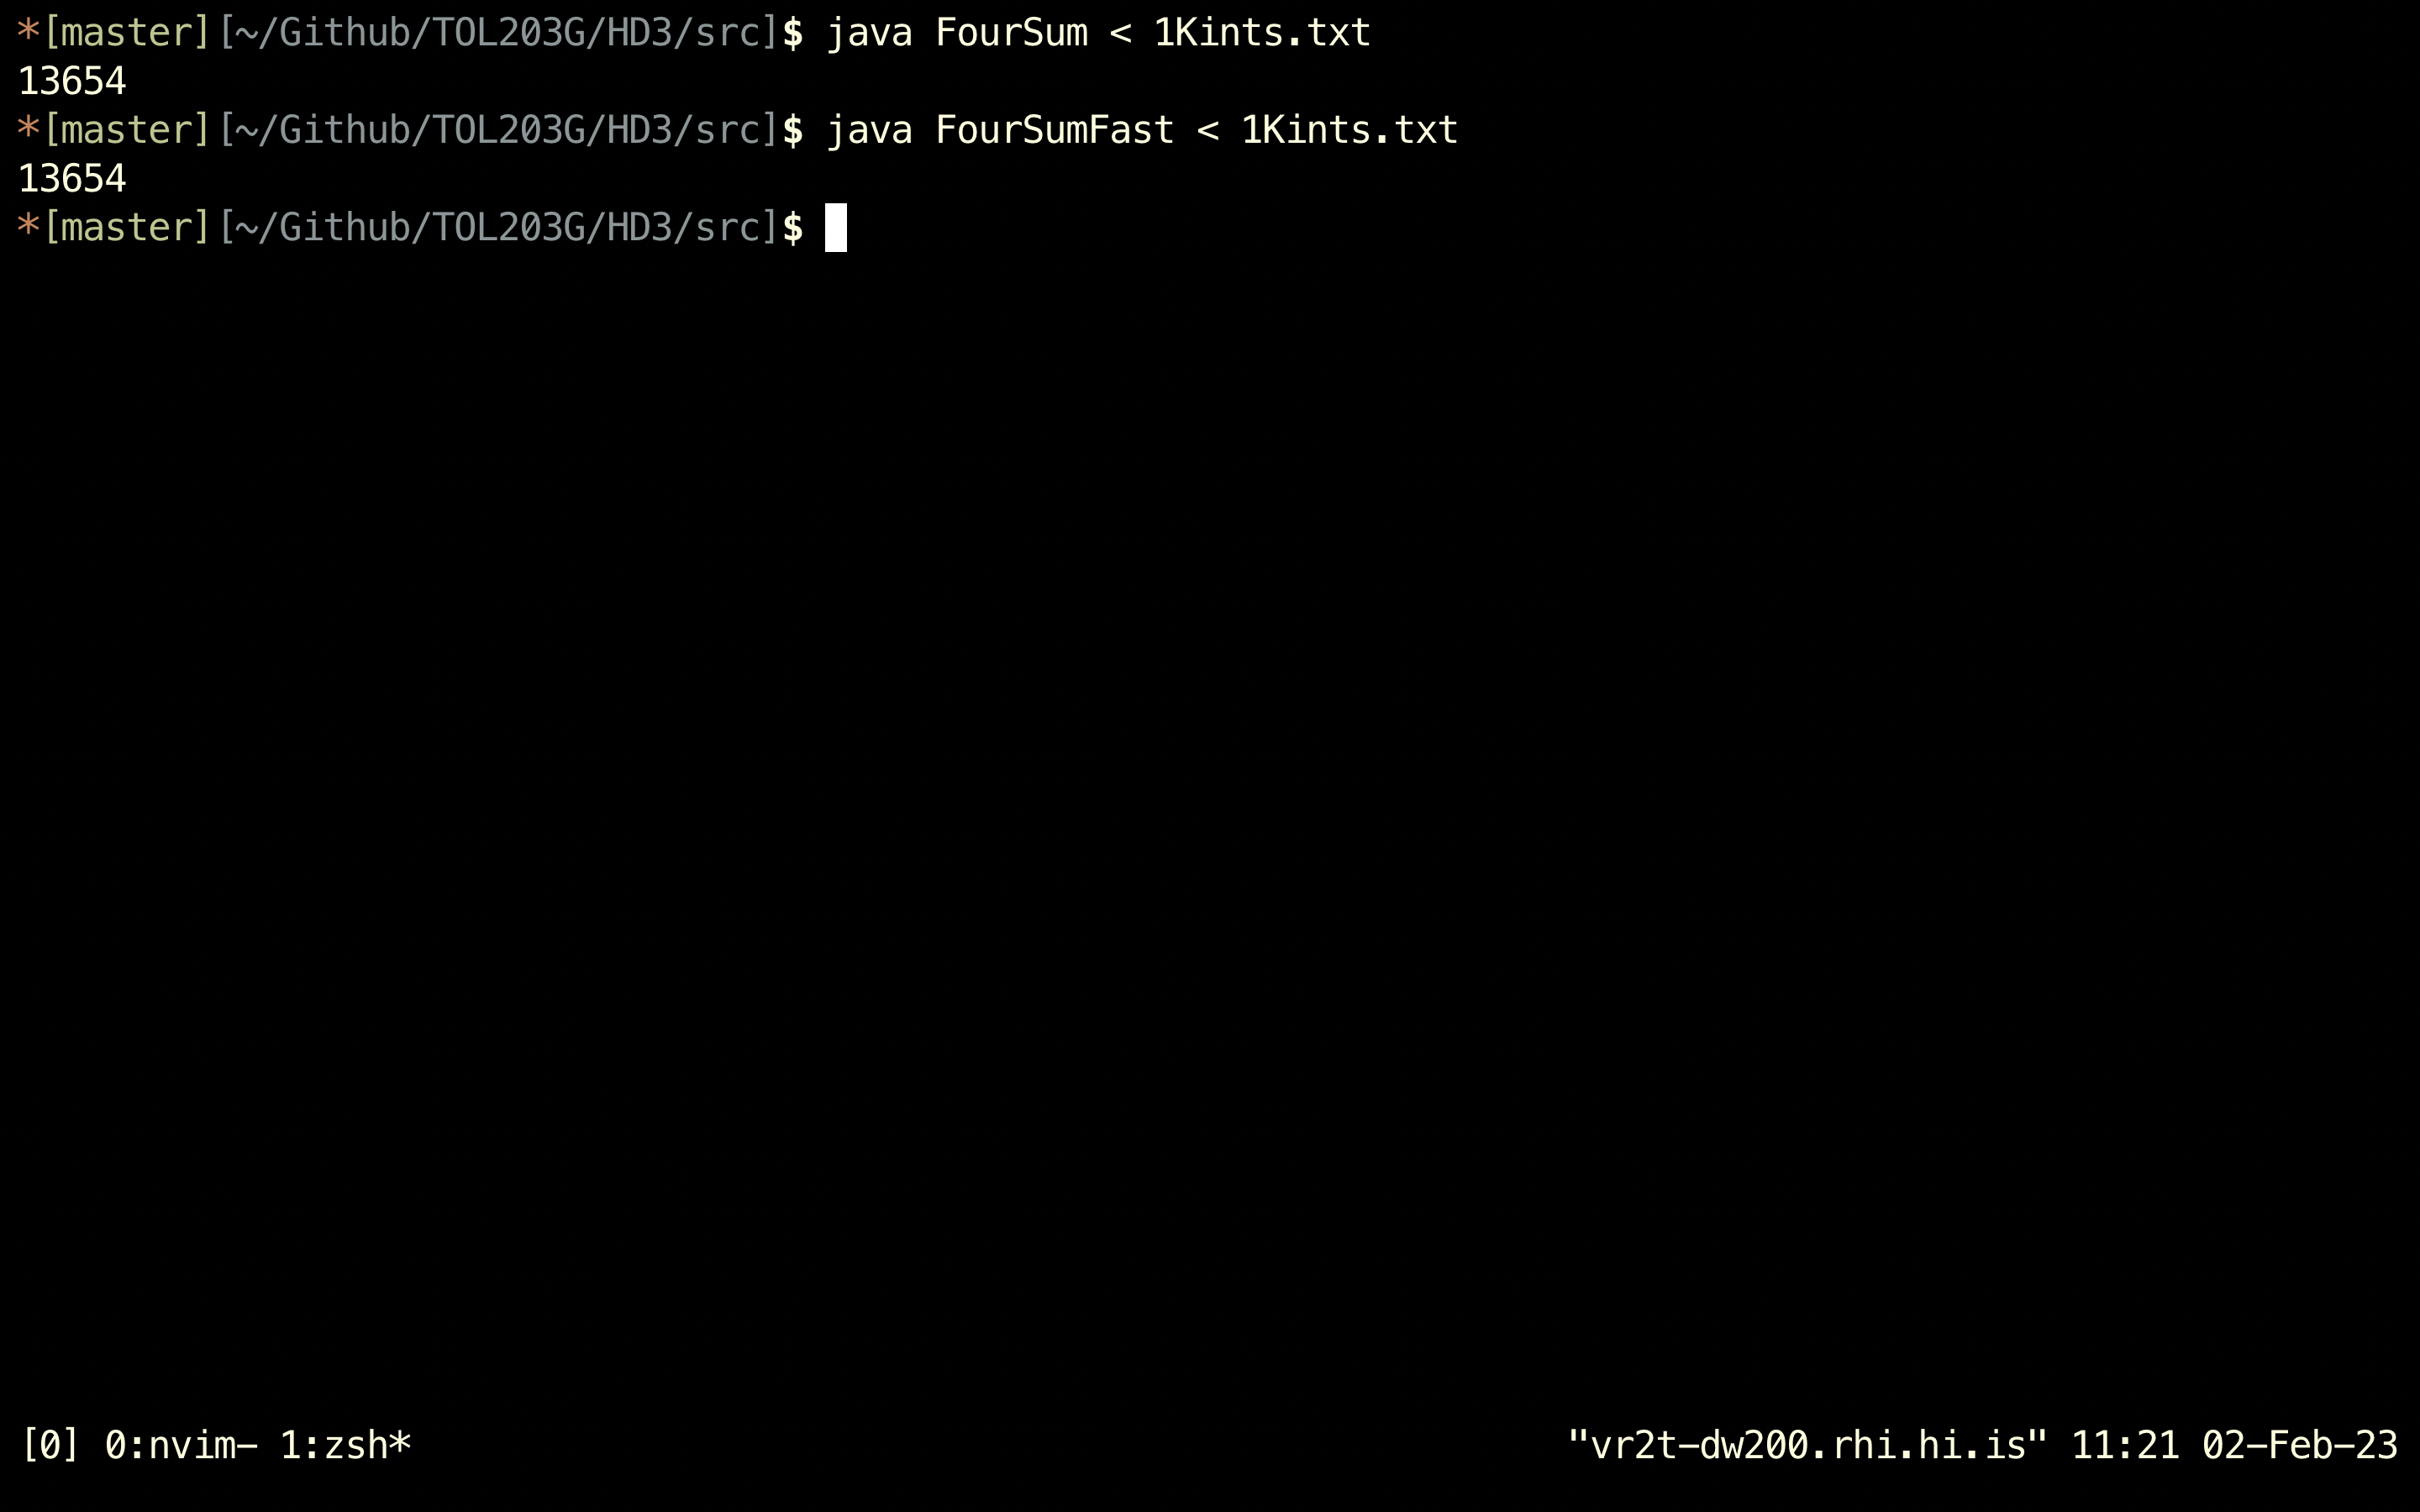
\includegraphics[width=\textwidth]{img/foursum_keyrsla.png} 
   \caption{Keyrsla \texttt{FourSum} og \texttt{FourSumFast} í skel}
   \label{mynd1}
\end{figure}

\noindent
Eins og má sjá fáum við 13654 sem er viðbúinn fjöldi fernda.

\newpage
\noindent
\textbf{\large Verkefni 2} \medskip \\
Framhald af æfingadæminu að ofan.
\begin{enumerate}[label=(\alph*)]
    \item Finnið raunhæf neðri mörk á vaxtarhraða keyrslutíma reiknirits sem leysir þetta verkefni, þ.e. hversu margar
    aðgerðir þurfa öll reiknirit að nota til þess að leysa þetta verkefni (sem fall af $N$)? Rökstyðjið svarið í nokkrum
    orðum.

    \item Það er hægt að leysa verkefnið á mun hraðvirkar hátt en gert var í æfingadæminu, með því að nýta sér fyrri útreikninga
    í $B$. Hugmyndin er þið eruð að reikna út \texttt{B[i,j]} þá eruð þið nýbúin að reikna út \texttt{B[i, j-1]}. Er ekki hægt að
    nota það gildi? Útfærið þetta reiknirit í Java og keyrið það fyrir sömu gildi á $N$ og gert var í æfingadæminu. Hver er vaxtarhraði
    þessa nýja reiknirits? Skilið kóðanum (sem texta, ekki skjáskoti) og svarinu.
\end{enumerate}

\medskip
\noindent
\textbf{\large Lausn} \medskip \\
\textbf{Hluti (a)} \medskip \\
Látum $\sigma(i, j) \coloneqq \sum_{k = i}^j a_k$.\footnote{Við notum hér bilið $1, \ldots, N$ í stað $0, \ldots, N-1$
eins og venja er fyrir í stærðfræðilegum rithætti fyrir runur. Þá er inntakið okkar heiltöluruna á forminu $a_1, \ldots, a_N$.} Við getum sett upp töflu sem sýnir hvernig
fylkið $B$ lítur út fyrir gefna inntaksstærð $N$:

\renewcommand{\arraystretch}{1.25}
\begin{table}[ht!]
    \centering
    \begin{tabular}{ccccc}
        \toprule
        $\downarrow$ i $\rightarrow$ j &  1 & 2 & $\cdots$ & N \\
        \midrule
        1        & $\sigma(1, 1)$ &— & $\cdots$ & — \\
        2        & $\sigma(2, 1)$ &$\sigma(2, 2)$ & $\cdots$ & — \\
        $\vdots$ & $\vdots$ & $\vdots$ & $\ddots$ & $\vdots$ \\
        $N$ & $\sigma(N, 1)$ & $\sigma(N, 2)$ & $\cdots$ & $\sigma(N, N)$ \\ 
        \bottomrule
    \end{tabular}
    \caption{Útlit fylkisins $B$.}
\end{table}

\noindent
Við miðum almenna kostanaðarlíkanið út frá fjölda fallakalla á $\sigma(i, j)$. Við sjáum
að heildafjöldi kalla er $1 + 2 + \cdots + N$ svo við fáum
\[
    T(N) = 1 + 2 + \cdots + N = \frac{N(N + 1)}{2} \sim \frac 12 N^2
\]
m.ö.o. er $T(N) \sim \Omega(N^2)$.

\newpage
\noindent
\textbf{Hluti (b)} \medskip \\
Við skulum hefja umfjöllunina á upprunalega fallinu. Ef við útfærum sauðakóðann
sem er gefinn í æfingadæminu í Java fáum við eftirfarandi forritsbút:

\begin{listing}[ht!]
    \centering
    \inputminted[firstline=13, lastline=22, linenos]{java}{../src/V2/ArraySum.java}
    \caption{Fallið \texttt{arraysum} (hægari útfærsla)}
    \label{forrit2}
\end{listing}

\noindent
Í þessari aðferð útfærum við hlutsummufallið $\sigma(i, j)$ með því að ítra í gegnum bilið
með $i \leq k \leq j$, sækja gildið $a_k$ hverju sinni og leggja við $b_{ij}$. Þessi aðferð
er línuleg, þ.e. kostnaður hennar er $N$ á heildina litið og því er tímaflækja þessa forritsbúts
$T(n) \sim \mathcal O(N^3)$.

Hin útfærslan er mun hraðvirkari. Hún gengur þannig fyrir sig að við ítrum sem áður í gegnum fylkið.
Ef við erum í hornalínustaki er það fyrsta stakið sem leggur eitthvað til summunnar og því setjum við
einfaldlega $B_{ij} = A_i$ ef $i = j$.\footnote{Þetta getur allt að eins verið $A_j$ því $A_i = A_j$ því $i = j$.} 
Ef svo er ekki þá setjum við $B_{ij} = B_{i, j-1} + A_j$ því við höfum þegar reiknað $B_{i, j-1}$. Forritsbúturinn er gefinn fyrir neðan:

\begin{listing}[ht!]
    \centering 
    \inputminted[firstline=31, lastline=39, linenos]{java}{../src/V2/ArraySum.java}
    \caption{Fallið \texttt{arraysum\_fast} (hraðari útfærsla)}
    \label{forrit3}
\end{listing}

\begin{figure}[ht!]
    \centering
    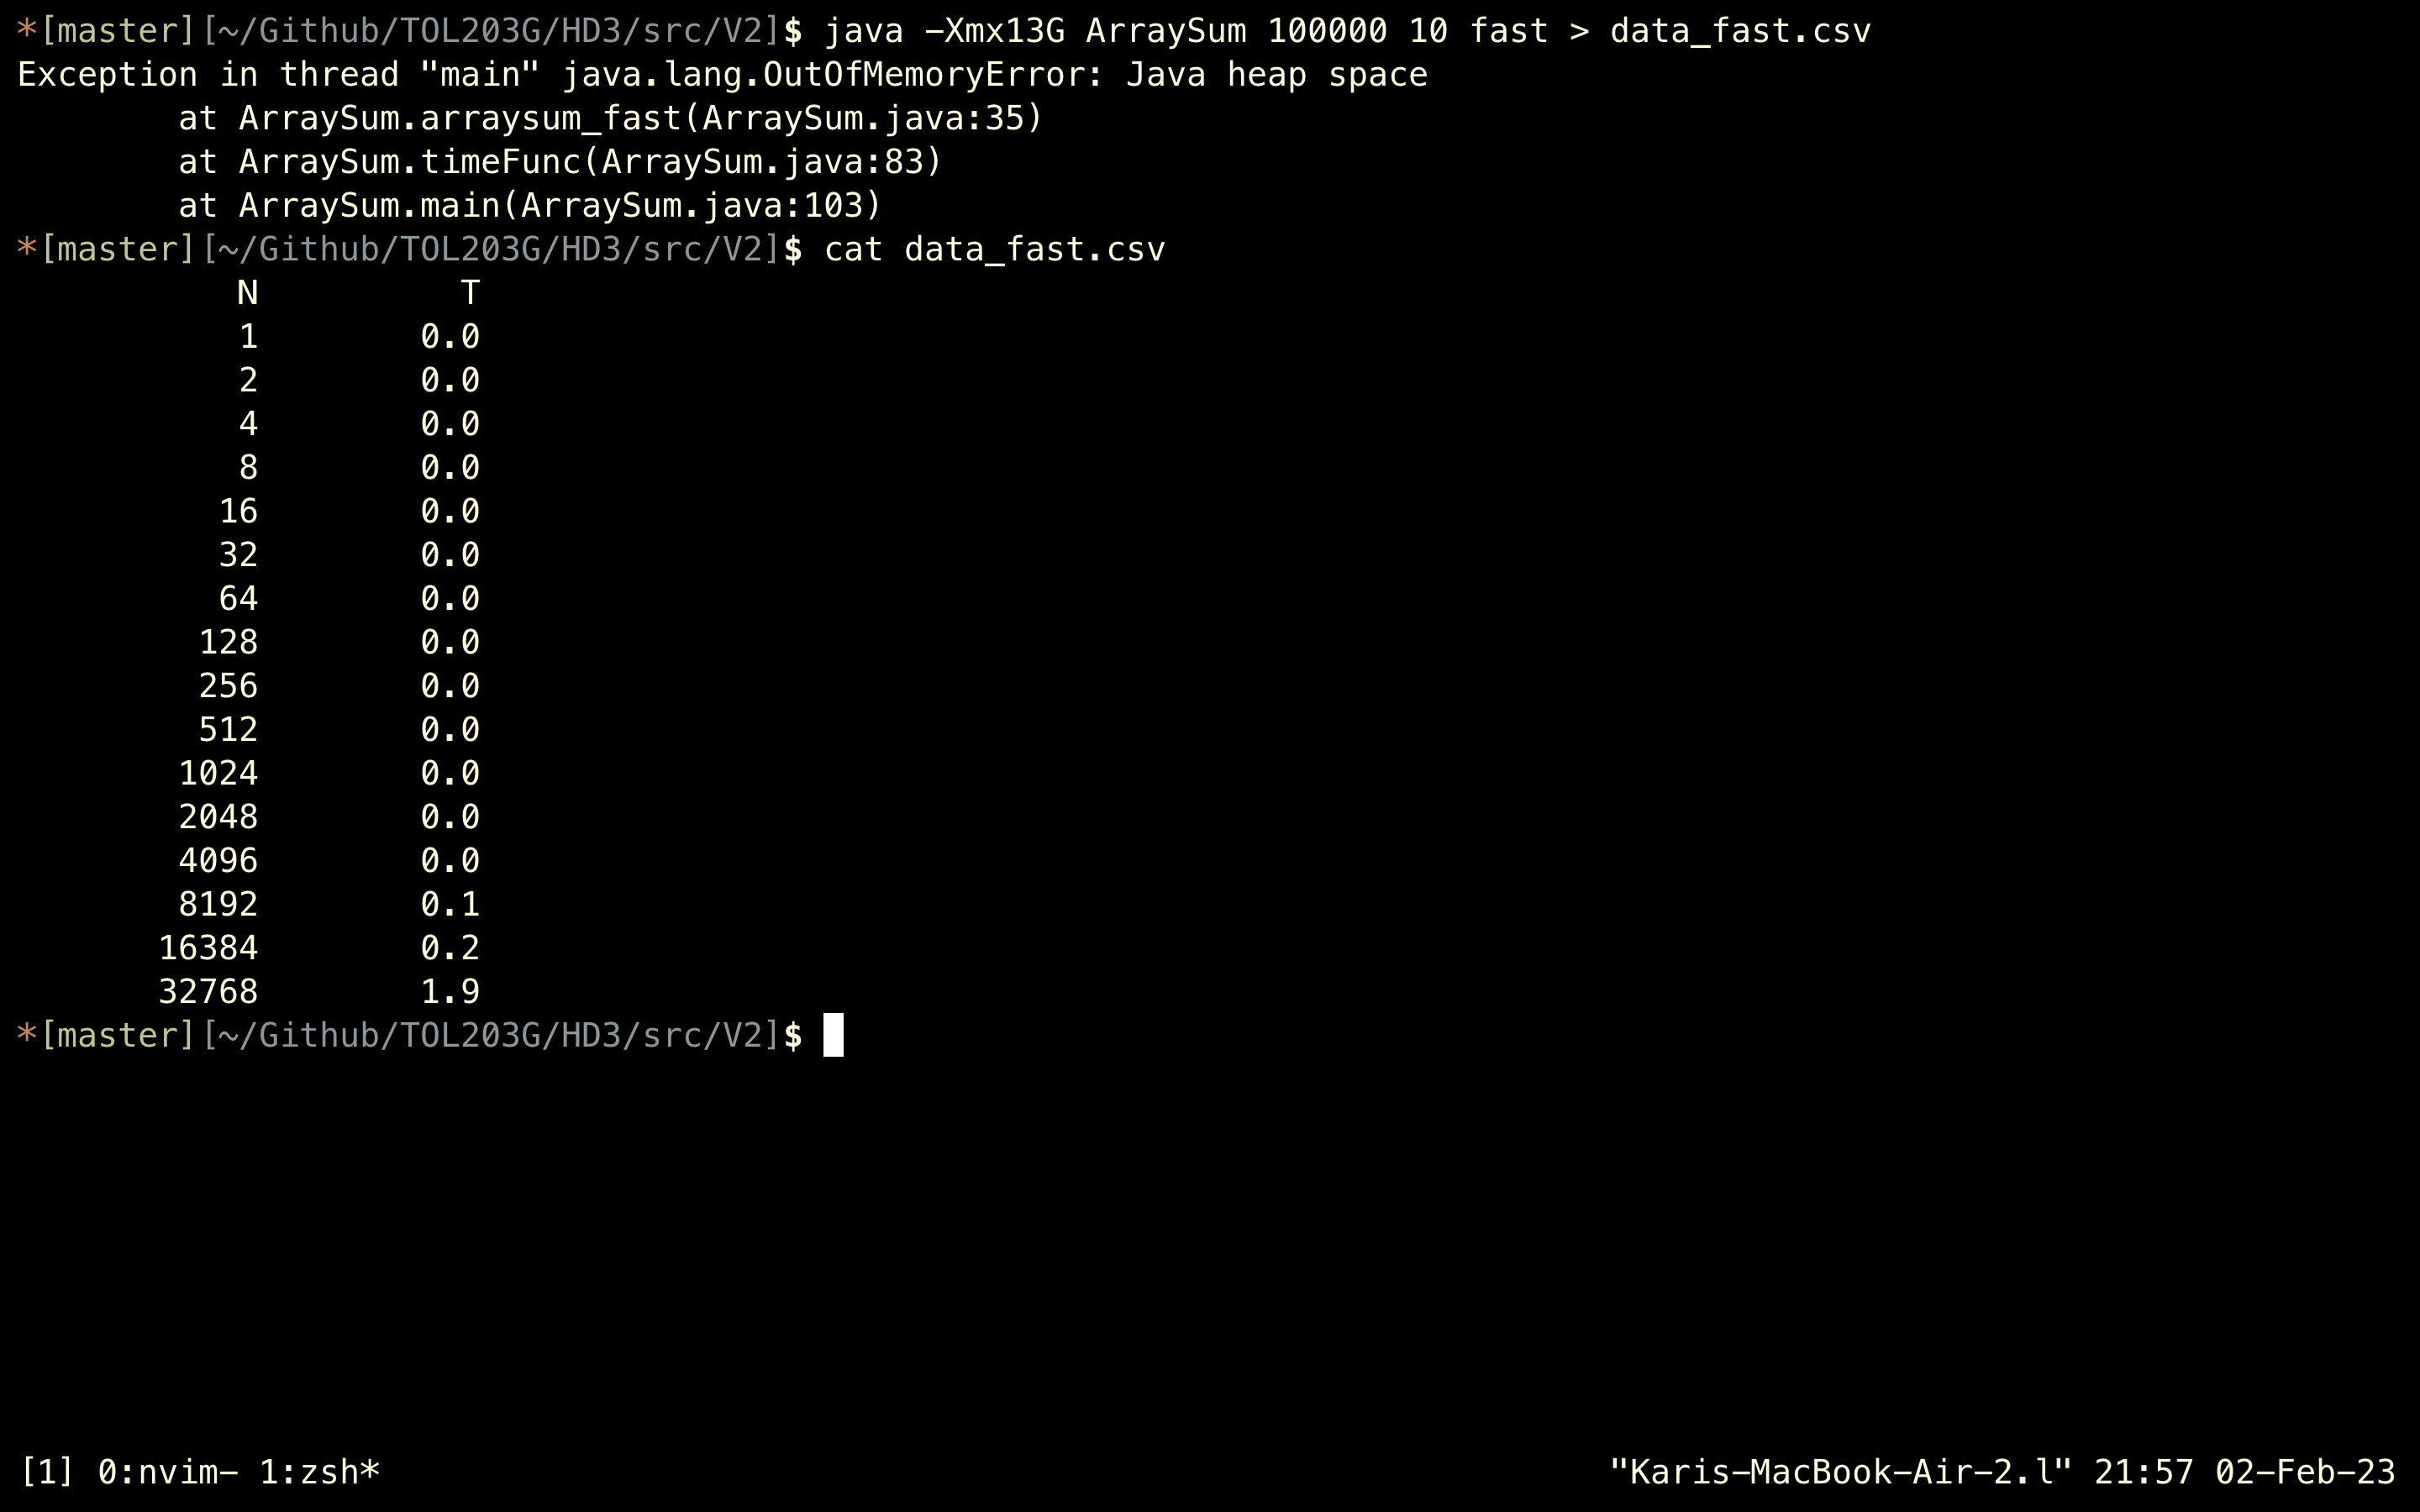
\includegraphics[width=\textwidth]{img/arraysum_keyrsla.png}
    \caption{Keyrsla á \texttt{ArraySum.java} og söfnun gagna}
\end{figure}

\noindent
Útfærslan í forriti \ref{forrit3} tryggir $\sigma(i, j) \sim \mathcal O(1)$ þ.e. summuaðgerðin er fasti hverju sinni svo við
búumst við því að $T(N) \sim \mathcal O(N^2)$ fyrir þessa útfærslu. Við göngum úr skugga um þetta með mælingum.

Látum $T_s(N)$ tákna tímaflækju meintu hægari útfærslunnar en $T_f(N)$ tákna meintu
hraðari útfærsluna. Við spáðum fyrir að $T_s(N) \sim \mathcal O(N^3)$ og að $T_f(N) \sim \mathcal O(N^2)$.
Við keyrum notendaforritið í skel og beinum staðalúttakinu í csv skrá til frekari úrvinnslu, eins og mynd fyrir neðan sýnir.

Mynd fyrir neðan sýnir keyrsluna á \texttt{ArraySum.java}. Notuð var stillingin \texttt{-Xmx13G} til að gefa forritinu $13$ GB
til keyrslu en þá getum við fengið aðeins meiri gögn. Hið sama var endurtekið á nýjan leik fyrir hægari útfærsluna. Útreiknað tvöföldunarhlutfall
fyrir hægu útfærsluna var $2.292 \approx 2$ en fyrir þá hröðu fékkst $2.832 \approx 3$. Þessu ber saman við tilgátu okkar.
Samanburður á keyrslutíma útfærslanna má sjá á mynd \ref{mynd3}.

\begin{figure}[ht!]
    \centering
    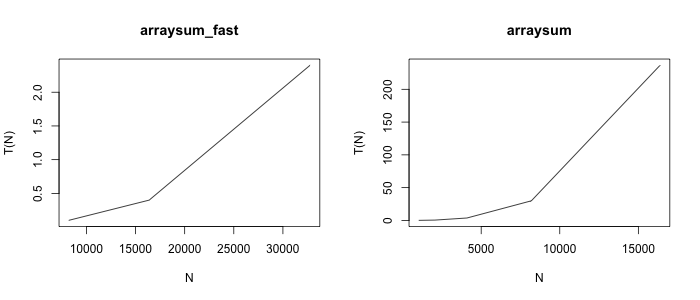
\includegraphics[width=\textwidth]{img/speed_comparison_nonlog.png}
    \caption{Keyrslutími á \texttt{arraysum} og \texttt{arraysum\_fast} eftir $N$}
    \label{mynd3}
\end{figure}


\newpage
\noindent
\textbf{\large Verkefni 3} \medskip \\
Tiltekið hótel hefur $N$ herbergi, sem eru í röð á löngum gangi. Herbergi $0$ er næst móttökunni, en herbergi $N-1$ er lengst í burtu.
Öll herbergin frá $0$ til $F-1$, en herbergi $F$ til $N-1$ eru laus. Við viljum sjálf vera í herbergi $F$, en við vitum ekki gildið á $F$
(aðeins að $F < N$). Til þess að finna fyrsta lausa herbergið getum við aðeins kannað eitt herbergi í einu með því að banka á hurðina og kíkja
inn. Við viljum lágmarka fjölda skipta sem við bönkum á hurðir í versta tilfelli.

\begin{enumerate}[label=(\alph*)]
    \item Hver er versta tilfellis tími (sem fall af $N$) á reikniriti sem byrjar á herbergi $0$ og rekur sig út eftir ganginum þar til fyrsta
    lausa herbergið er fundið?
    \item Lýsið reikniriti sem notar í versta falli $\log N$ tíma til að finna fyrsta lausa herbergið.
    \item Ef $N$ er mikið stærra en $F$, þá er hægt að gera betur og nota aðeins $\sim 2 \log F$ tíma til þess að finna fyrsta lausa herbergið.
    Lýsið þessari aðferð og rökstyðjið vaxtarhraða hennar.
\end{enumerate}

\medskip
\noindent
\textbf{\large Lausn} \medskip \\
\textbf{Hluti (a)} \medskip \\
Ef við gefum okkur að aðferðin er að fara hurð eftir hurð eftir ganginum fæst versta tilfellið þegar
$F = N-1$. Þá er tímaflækjan nokkurn veginn $\sim N$.

\newpage
\noindent
\textbf{Hluti (b)} \medskip \\
Til þess að útfæra þetta notum við afbrigði af binary search. Java forritið er fyrir neðan:

\begin{listing}[ht!]
    \centering
    \inputminted[firstline=5, lastline=18, linenos]{java}{../src/V3/HotelRoom.java}
    \caption{Fallið \texttt{find\_room}}
\end{listing}

\noindent
Þetta forrit notar binary search og tímaflækja þess er því $T(N) \sim \mathcal O(\lg N)$.

\medskip
\noindent
\textbf{Hluti (c)} \medskip \\
Gefið er að $F$ sé mun minna en $N$. Aðferðin sem við notum hér er að byrja frá núlli og rekja okkur
með tvöföldun þangað til við komum að tómu hólfi. Til að vera viss um að við séum örugglega í $F$ keyrum
við síðan helmingunarleit á þessu bili. Heildarkostnaðurinn er $\lg F + \lg F =  2\lg F$.

\newpage
\noindent
\textbf{\large Verkefni 4} \medskip \\
Geta eftirfarandi \texttt{id[]} fylki komið út þegar reikniritið vigtað \emph{Quick-union}
án vegþjöppunar er keyrt með $N = 8$? Teiknið upp trén í hvoru tilfelli og útskýrið hvers vegna
þetta fylki er ómögulegt eða sýnið röð \emph{union}-aðgerða sem enda í þessu fylki.

\begin{enumerate}[label=(\alph*)]
    \item 0, 1, 0, 3, 1, 1, 1, 3
    \item 5, 0, 6, 6, 5, 6, 6, 4
\end{enumerate}

\medskip
\noindent
\textbf{\large Lausn} \medskip \\
\textbf{Hluti (a)} \medskip \\
Það er hægt að mynda þetta fylki með eftirfarandi runu aðgerða:
$\texttt{union}(2,0) \to \texttt{union}(4,1) \to \texttt{union}(5,1) \to \texttt{union}(6,1) \to \texttt{union}(7,3)$.
Sjá mynd 4.



\tikzset{every picture/.style={line width=0.75pt}} %set default line width to 0.75pt        

\begin{figure}[ht!]
    \centering
    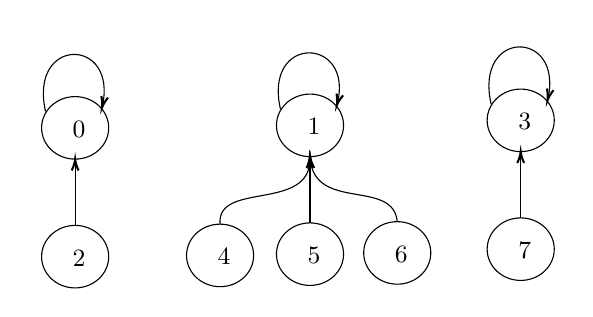
\begin{tikzpicture}[x=0.75pt,y=0.75pt,yscale=-0.5,xscale=.5]
    %uncomment if require: \path (0,310); %set diagram left start at 0, and has height of 310

    %Shape: Ellipse [id:dp24329331479239147] 
    \draw   (96,225.38) .. controls (96,208.74) and (110.47,195.25) .. (128.33,195.25) .. controls (146.19,195.25) and (160.66,208.74) .. (160.66,225.38) .. controls (160.66,242.01) and (146.19,255.5) .. (128.33,255.5) .. controls (110.47,255.5) and (96,242.01) .. (96,225.38) -- cycle ;

    %Shape: Ellipse [id:dp4576600602165295] 
    \draw   (96,101.27) .. controls (96,84.63) and (110.47,71.14) .. (128.33,71.14) .. controls (146.19,71.14) and (160.66,84.63) .. (160.66,101.27) .. controls (160.66,117.9) and (146.19,131.39) .. (128.33,131.39) .. controls (110.47,131.39) and (96,117.9) .. (96,101.27) -- cycle ;
    %Straight Lines [id:da10105715175879992] 
    \draw    (128.33,195.25) -- (128.33,133.39) ;
    \draw [shift={(128.33,131.39)}, rotate = 90] [color={rgb, 255:red, 0; green, 0; blue, 0 }  ][line width=0.75]    (10.93,-3.29) .. controls (6.95,-1.4) and (3.31,-0.3) .. (0,0) .. controls (3.31,0.3) and (6.95,1.4) .. (10.93,3.29)   ;
    %Curve Lines [id:da1994001120256197] 
    \draw    (99.85,85.62) .. controls (83.12,12.49) and (170.1,13.31) .. (154.41,80.98) ;
    \draw [shift={(154.16,82)}, rotate = 283.75] [color={rgb, 255:red, 0; green, 0; blue, 0 }  ][line width=0.75]    (10.93,-3.29) .. controls (6.95,-1.4) and (3.31,-0.3) .. (0,0) .. controls (3.31,0.3) and (6.95,1.4) .. (10.93,3.29)   ;
    %Shape: Ellipse [id:dp033453599676222634] 
    \draw   (322.31,222.97) .. controls (322.31,206.33) and (336.78,192.84) .. (354.64,192.84) .. controls (372.49,192.84) and (386.97,206.33) .. (386.97,222.97) .. controls (386.97,239.6) and (372.49,253.09) .. (354.64,253.09) .. controls (336.78,253.09) and (322.31,239.6) .. (322.31,222.97) -- cycle ;
    %Shape: Ellipse [id:dp9300638239423946] 
    \draw   (322.31,98.86) .. controls (322.31,82.22) and (336.78,68.73) .. (354.64,68.73) .. controls (372.49,68.73) and (386.97,82.22) .. (386.97,98.86) .. controls (386.97,115.49) and (372.49,128.98) .. (354.64,128.98) .. controls (336.78,128.98) and (322.31,115.49) .. (322.31,98.86) -- cycle ;
    %Straight Lines [id:da4217377367889521] 
    \draw    (354.64,192.84) -- (354.64,130.98) ;
    \draw [shift={(354.64,128.98)}, rotate = 90] [color={rgb, 255:red, 0; green, 0; blue, 0 }  ][line width=0.75]    (10.93,-3.29) .. controls (6.95,-1.4) and (3.31,-0.3) .. (0,0) .. controls (3.31,0.3) and (6.95,1.4) .. (10.93,3.29)   ;
    %Curve Lines [id:da6820917331833274] 
    \draw    (326.16,83.21) .. controls (309.43,10.08) and (397.86,13.29) .. (380.74,78.61) ;
    \draw [shift={(380.47,79.6)}, rotate = 285.42] [color={rgb, 255:red, 0; green, 0; blue, 0 }  ][line width=0.75]    (10.93,-3.29) .. controls (6.95,-1.4) and (3.31,-0.3) .. (0,0) .. controls (3.31,0.3) and (6.95,1.4) .. (10.93,3.29)   ;
    %Shape: Ellipse [id:dp6937445946747205] 
    \draw   (235.66,224.17) .. controls (235.66,207.53) and (250.14,194.05) .. (267.99,194.05) .. controls (285.85,194.05) and (300.32,207.53) .. (300.32,224.17) .. controls (300.32,240.81) and (285.85,254.3) .. (267.99,254.3) .. controls (250.14,254.3) and (235.66,240.81) .. (235.66,224.17) -- cycle ;
    %Curve Lines [id:da7780602984900371] 
    \draw    (267.99,194.05) .. controls (264.23,152.31) and (355.45,182.6) .. (354.69,130.58) ;
    \draw [shift={(354.64,128.98)}, rotate = 87.19] [color={rgb, 255:red, 0; green, 0; blue, 0 }  ][line width=0.75]    (10.93,-3.29) .. controls (6.95,-1.4) and (3.31,-0.3) .. (0,0) .. controls (3.31,0.3) and (6.95,1.4) .. (10.93,3.29)   ;
    %Shape: Ellipse [id:dp5361630916414397] 
    \draw   (406.37,221.76) .. controls (406.37,205.12) and (420.84,191.64) .. (438.7,191.64) .. controls (456.55,191.64) and (471.03,205.12) .. (471.03,221.76) .. controls (471.03,238.4) and (456.55,251.89) .. (438.7,251.89) .. controls (420.84,251.89) and (406.37,238.4) .. (406.37,221.76) -- cycle ;
    %Curve Lines [id:da6470432187410788] 
    \draw    (438.7,191.64) .. controls (434.93,149.9) and (358.85,182.55) .. (354.74,130.58) ;
    \draw [shift={(354.64,128.98)}, rotate = 87.19] [color={rgb, 255:red, 0; green, 0; blue, 0 }  ][line width=0.75]    (10.93,-3.29) .. controls (6.95,-1.4) and (3.31,-0.3) .. (0,0) .. controls (3.31,0.3) and (6.95,1.4) .. (10.93,3.29)   ;
    %Shape: Ellipse [id:dp24180222349913771] 
    \draw   (525.34,218.15) .. controls (525.34,201.51) and (539.81,188.02) .. (557.67,188.02) .. controls (575.53,188.02) and (590,201.51) .. (590,218.15) .. controls (590,234.78) and (575.53,248.27) .. (557.67,248.27) .. controls (539.81,248.27) and (525.34,234.78) .. (525.34,218.15) -- cycle ;
    %Shape: Ellipse [id:dp39739191437804866] 
    \draw   (525.34,94.04) .. controls (525.34,77.4) and (539.81,63.91) .. (557.67,63.91) .. controls (575.53,63.91) and (590,77.4) .. (590,94.04) .. controls (590,110.67) and (575.53,124.16) .. (557.67,124.16) .. controls (539.81,124.16) and (525.34,110.67) .. (525.34,94.04) -- cycle ;
    %Straight Lines [id:da7583938364324243] 
    \draw    (557.67,188.02) -- (557.67,126.16) ;
    \draw [shift={(557.67,124.16)}, rotate = 90] [color={rgb, 255:red, 0; green, 0; blue, 0 }  ][line width=0.75]    (10.93,-3.29) .. controls (6.95,-1.4) and (3.31,-0.3) .. (0,0) .. controls (3.31,0.3) and (6.95,1.4) .. (10.93,3.29)   ;
    %Curve Lines [id:da9520394001845716] 
    \draw    (529.19,78.39) .. controls (512.46,5.26) and (599.44,6.08) .. (583.75,73.75) ;
    \draw [shift={(583.5,74.78)}, rotate = 283.75] [color={rgb, 255:red, 0; green, 0; blue, 0 }  ][line width=0.75]    (10.93,-3.29) .. controls (6.95,-1.4) and (3.31,-0.3) .. (0,0) .. controls (3.31,0.3) and (6.95,1.4) .. (10.93,3.29)   ;

    \small
    % Text Node
    \draw (123.48,216.38) node [anchor=north west][inner sep=0.75pt]   [align=left] {$\displaystyle 2$};
    % Text Node
    \draw (123.48,92.27) node [anchor=north west][inner sep=0.75pt]   [align=left] {$\displaystyle 0$};
    % Text Node
    \draw (349.79,89.86) node [anchor=north west][inner sep=0.75pt]   [align=left] {$\displaystyle 1$};
    % Text Node
    \draw (349.79,213.97) node [anchor=north west][inner sep=0.75pt]   [align=left] {$\displaystyle 5$};
    % Text Node
    \draw (263.14,215.17) node [anchor=north west][inner sep=0.75pt]   [align=left] {$\displaystyle 4$};
    % Text Node
    \draw (433.84,212.76) node [anchor=north west][inner sep=0.75pt]   [align=left] {$\displaystyle 6$};
    % Text Node
    \draw (552.82,85.04) node [anchor=north west][inner sep=0.75pt]   [align=left] {$\displaystyle 3$};
    % Text Node
    \draw (552.82,209.15) node [anchor=north west][inner sep=0.75pt]   [align=left] {$\displaystyle 7$};
    \end{tikzpicture}
    \caption{Tréð úr (a)-hluta}
\end{figure}

\medskip
\noindent
\textbf{Hluti (b)} \medskip \\
Það er ekki hægt að mynda þetta tré. Í seinustu aðgerðinni er samhengisþátturinn 5
þyngri en 6 og því myndi 6 eignast 5 sem rót. Sjá mynd 5.


\begin{figure}[ht!]
    \centering
    \tikzset{every picture/.style={line width=0.75pt}} %set default line width to 0.75pt        
    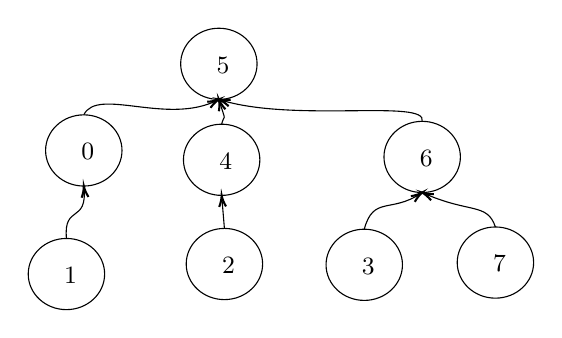
\begin{tikzpicture}[x=0.75pt,y=0.75pt,yscale=-.5,xscale=.5]
        %uncomment if require: \path (0,310); %set diagram left start at 0, and has height of 310
        
        %Shape: Ellipse [id:dp24329331479239147] 
        \draw   (249.54,240.04) .. controls (249.54,221.1) and (266.02,205.74) .. (286.35,205.74) .. controls (306.68,205.74) and (323.16,221.1) .. (323.16,240.04) .. controls (323.16,258.99) and (306.68,274.34) .. (286.35,274.34) .. controls (266.02,274.34) and (249.54,258.99) .. (249.54,240.04) -- cycle ;
        
        %Shape: Ellipse [id:dp010405702732570576] 
        \draw   (114.04,130.61) .. controls (114.04,111.66) and (130.52,96.31) .. (150.85,96.31) .. controls (171.18,96.31) and (187.66,111.66) .. (187.66,130.61) .. controls (187.66,149.55) and (171.18,164.91) .. (150.85,164.91) .. controls (130.52,164.91) and (114.04,149.55) .. (114.04,130.61) -- cycle ;
        
        %Shape: Ellipse [id:dp34146645914089735] 
        \draw   (244.2,47.14) .. controls (244.2,28.2) and (260.68,12.84) .. (281.01,12.84) .. controls (301.34,12.84) and (317.82,28.2) .. (317.82,47.14) .. controls (317.82,66.09) and (301.34,81.44) .. (281.01,81.44) .. controls (260.68,81.44) and (244.2,66.09) .. (244.2,47.14) -- cycle ;
        
        %Shape: Ellipse [id:dp4315236170324319] 
        \draw   (97.31,249.7) .. controls (97.31,230.76) and (113.79,215.4) .. (134.12,215.4) .. controls (154.45,215.4) and (170.93,230.76) .. (170.93,249.7) .. controls (170.93,268.64) and (154.45,284) .. (134.12,284) .. controls (113.79,284) and (97.31,268.64) .. (97.31,249.7) -- cycle ;
        
        %Shape: Ellipse [id:dp5112632145651108] 
        \draw   (246.88,139.61) .. controls (246.88,120.66) and (263.36,105.31) .. (283.69,105.31) .. controls (304.02,105.31) and (320.5,120.66) .. (320.5,139.61) .. controls (320.5,158.55) and (304.02,173.91) .. (283.69,173.91) .. controls (263.36,173.91) and (246.88,158.55) .. (246.88,139.61) -- cycle ;
        
        %Shape: Ellipse [id:dp6552328651074013] 
        \draw   (440.11,136.86) .. controls (440.11,117.92) and (456.59,102.56) .. (476.92,102.56) .. controls (497.25,102.56) and (513.73,117.92) .. (513.73,136.86) .. controls (513.73,155.81) and (497.25,171.16) .. (476.92,171.16) .. controls (456.59,171.16) and (440.11,155.81) .. (440.11,136.86) -- cycle ;
        
        %Shape: Ellipse [id:dp6183835565611506] 
        \draw   (510.68,238.64) .. controls (510.68,219.7) and (527.16,204.34) .. (547.49,204.34) .. controls (567.82,204.34) and (584.3,219.7) .. (584.3,238.64) .. controls (584.3,257.59) and (567.82,272.94) .. (547.49,272.94) .. controls (527.16,272.94) and (510.68,257.59) .. (510.68,238.64) -- cycle ;
        
        %Shape: Ellipse [id:dp12252929155283354] 
        \draw   (384.29,240.8) .. controls (384.29,221.85) and (400.77,206.5) .. (421.1,206.5) .. controls (441.43,206.5) and (457.91,221.85) .. (457.91,240.8) .. controls (457.91,259.74) and (441.43,275.1) .. (421.1,275.1) .. controls (400.77,275.1) and (384.29,259.74) .. (384.29,240.8) -- cycle ;
        
        %Curve Lines [id:da5582133667456155] 
        \draw    (150.85,96.31) .. controls (163.93,69.11) and (231.11,106.78) .. (279.55,82.21) ;
        \draw [shift={(281.01,81.44)}, rotate = 151.73] [color={rgb, 255:red, 0; green, 0; blue, 0 }  ][line width=0.75]    (10.93,-3.29) .. controls (6.95,-1.4) and (3.31,-0.3) .. (0,0) .. controls (3.31,0.3) and (6.95,1.4) .. (10.93,3.29)   ;
        %Curve Lines [id:da6262026827422038] 
        \draw    (134.12,215.4) .. controls (131.18,182.07) and (154.34,201.45) .. (151.02,166.54) ;
        \draw [shift={(150.85,164.91)}, rotate = 83.55] [color={rgb, 255:red, 0; green, 0; blue, 0 }  ][line width=0.75]    (10.93,-3.29) .. controls (6.95,-1.4) and (3.31,-0.3) .. (0,0) .. controls (3.31,0.3) and (6.95,1.4) .. (10.93,3.29)   ;
        %Straight Lines [id:da23544085906916323] 
        \draw    (286.35,205.74) -- (283.86,175.9) ;
        \draw [shift={(283.69,173.91)}, rotate = 85.23] [color={rgb, 255:red, 0; green, 0; blue, 0 }  ][line width=0.75]    (10.93,-3.29) .. controls (6.95,-1.4) and (3.31,-0.3) .. (0,0) .. controls (3.31,0.3) and (6.95,1.4) .. (10.93,3.29)   ;
        %Curve Lines [id:da12282341880585435] 
        \draw    (283.69,105.31) .. controls (286.28,94.17) and (288.51,105.8) .. (281.56,83.25) ;
        \draw [shift={(281.01,81.44)}, rotate = 73.04] [color={rgb, 255:red, 0; green, 0; blue, 0 }  ][line width=0.75]    (10.93,-3.29) .. controls (6.95,-1.4) and (3.31,-0.3) .. (0,0) .. controls (3.31,0.3) and (6.95,1.4) .. (10.93,3.29)   ;
        %Curve Lines [id:da2439501421887691] 
        \draw    (476.92,102.56) .. controls (482.79,80.64) and (353.18,104.21) .. (282.08,81.79) ;
        \draw [shift={(281.01,81.44)}, rotate = 17.98] [color={rgb, 255:red, 0; green, 0; blue, 0 }  ][line width=0.75]    (10.93,-3.29) .. controls (6.95,-1.4) and (3.31,-0.3) .. (0,0) .. controls (3.31,0.3) and (6.95,1.4) .. (10.93,3.29)   ;
        %Curve Lines [id:da9086624130665522] 
        \draw    (421.1,206.5) .. controls (429.96,174.08) and (446.67,191.27) .. (475.59,172.07) ;
        \draw [shift={(476.92,171.16)}, rotate = 145.24] [color={rgb, 255:red, 0; green, 0; blue, 0 }  ][line width=0.75]    (10.93,-3.29) .. controls (6.95,-1.4) and (3.31,-0.3) .. (0,0) .. controls (3.31,0.3) and (6.95,1.4) .. (10.93,3.29)   ;
        %Curve Lines [id:da7607811783372596] 
        \draw    (547.49,204.34) .. controls (539.49,180.66) and (522.67,191.58) .. (478.28,171.77) ;
        \draw [shift={(476.92,171.16)}, rotate = 24.45] [color={rgb, 255:red, 0; green, 0; blue, 0 }  ][line width=0.75]    (10.93,-3.29) .. controls (6.95,-1.4) and (3.31,-0.3) .. (0,0) .. controls (3.31,0.3) and (6.95,1.4) .. (10.93,3.29)   ;
        
        \small
        % Text Node
        \draw (281.59,231.04) node [anchor=north west][inner sep=0.75pt]   [align=left] {$\displaystyle 2$};
        % Text Node
        \draw (146.09,121.61) node [anchor=north west][inner sep=0.75pt]   [align=left] {$\displaystyle 0$};
        % Text Node
        \draw (129.36,240.7) node [anchor=north west][inner sep=0.75pt]   [align=left] {$\displaystyle 1$};
        % Text Node
        \draw (416.33,231.8) node [anchor=north west][inner sep=0.75pt]   [align=left] {$\displaystyle 3$};
        % Text Node
        \draw (278.93,130.61) node [anchor=north west][inner sep=0.75pt]   [align=left] {$\displaystyle 4$};
        % Text Node
        \draw (276.24,38.14) node [anchor=north west][inner sep=0.75pt]   [align=left] {$\displaystyle 5$};
        % Text Node
        \draw (472.16,127.86) node [anchor=north west][inner sep=0.75pt]   [align=left] {$\displaystyle 6$};
        % Text Node
        \draw (542.72,229.64) node [anchor=north west][inner sep=0.75pt]   [align=left] {$\displaystyle 7$};
        
        
    \end{tikzpicture}
    \caption{Tréð úr (b)-hluta}
    \label{mynd5}
\end{figure}


\newpage
\noindent
\textbf{\large Verkefni 5} \medskip \\
Í aðalútfærslunni á \emph{Union-find} í kennslubókinni, \texttt{UF.java}, er
notuð vegþjöppun með helmingun (\emph{path halving}). Rekjið ykkur í gegnum kóðann
í \texttt{UF.java} fyrir eftirfarandi sameiningar. Fjöldi staka er 6 og aðgerðirnar eru:
\[
    \texttt{union}(0,1) \to \texttt{union}(2,3) \to \texttt{union}(4,5) \to \texttt{union}(1,3) \to \texttt{union}(3,5)
\]
Teiknið trén eftir tvær síðustu aðgerðirnar og bendið á hvar raunveruleg vegþjöppun á sér stað
(þ.e. vegur í rótina styttist). Athugið að inni í hverri \emph{union}-aðgerð eru tvær \emph{find}-aðgerðir.

\medskip
\noindent
\textbf{\large Lausn} \medskip \\
Sjá mynd fyrir neðan.

\begin{figure}[ht!]
    \centering

    \tikzset{every picture/.style={line width=0.75pt}} %set default line width to 0.75pt        

    \begin{tikzpicture}[x=0.75pt,y=0.75pt,yscale=-1,xscale=1]
    %uncomment if require: \path (0,293); %set diagram left start at 0, and has height of 293

    %Shape: Ellipse [id:dp2810017048432343] 
    \draw   (91.2,98.58) .. controls (91.2,88.49) and (99.38,80.32) .. (109.46,80.32) .. controls (119.55,80.32) and (127.72,88.49) .. (127.72,98.58) .. controls (127.72,108.66) and (119.55,116.84) .. (109.46,116.84) .. controls (99.38,116.84) and (91.2,108.66) .. (91.2,98.58) -- cycle ;

    %Shape: Ellipse [id:dp8003298734509168] 
    \draw   (167.9,45.99) .. controls (167.9,35.91) and (176.07,27.73) .. (186.16,27.73) .. controls (196.24,27.73) and (204.42,35.91) .. (204.42,45.99) .. controls (204.42,56.08) and (196.24,64.25) .. (186.16,64.25) .. controls (176.07,64.25) and (167.9,56.08) .. (167.9,45.99) -- cycle ;

    %Shape: Ellipse [id:dp43069977365944245] 
    \draw   (169.36,97.12) .. controls (169.36,87.03) and (177.53,78.86) .. (187.62,78.86) .. controls (197.7,78.86) and (205.88,87.03) .. (205.88,97.12) .. controls (205.88,107.2) and (197.7,115.38) .. (187.62,115.38) .. controls (177.53,115.38) and (169.36,107.2) .. (169.36,97.12) -- cycle ;

    %Shape: Ellipse [id:dp5698767021303088] 
    \draw   (246.78,45.26) .. controls (246.78,35.18) and (254.95,27) .. (265.04,27) .. controls (275.12,27) and (283.3,35.18) .. (283.3,45.26) .. controls (283.3,55.34) and (275.12,63.52) .. (265.04,63.52) .. controls (254.95,63.52) and (246.78,55.34) .. (246.78,45.26) -- cycle ;

    %Shape: Ellipse [id:dp501228709657076] 
    \draw   (247.51,97.12) .. controls (247.51,87.03) and (255.69,78.86) .. (265.77,78.86) .. controls (275.85,78.86) and (284.03,87.03) .. (284.03,97.12) .. controls (284.03,107.2) and (275.85,115.38) .. (265.77,115.38) .. controls (255.69,115.38) and (247.51,107.2) .. (247.51,97.12) -- cycle ;

    %Shape: Ellipse [id:dp4965579946305667] 
    \draw   (92.66,46.72) .. controls (92.66,36.64) and (100.84,28.46) .. (110.92,28.46) .. controls (121.01,28.46) and (129.18,36.64) .. (129.18,46.72) .. controls (129.18,56.81) and (121.01,64.98) .. (110.92,64.98) .. controls (100.84,64.98) and (92.66,56.81) .. (92.66,46.72) -- cycle ;

    %Straight Lines [id:da19351268367756025] 
    \draw    (109.46,80.32) -- (110.1,66.98) ;
    \draw [shift={(110.19,64.98)}, rotate = 92.73] [color={rgb, 255:red, 0; green, 0; blue, 0 }  ][line width=0.75]    (10.93,-3.29) .. controls (6.95,-1.4) and (3.31,-0.3) .. (0,0) .. controls (3.31,0.3) and (6.95,1.4) .. (10.93,3.29)   ;
    %Straight Lines [id:da6298550679234696] 
    \draw    (187.62,78.86) -- (186.35,66.24) ;
    \draw [shift={(186.16,64.25)}, rotate = 84.29] [color={rgb, 255:red, 0; green, 0; blue, 0 }  ][line width=0.75]    (10.93,-3.29) .. controls (6.95,-1.4) and (3.31,-0.3) .. (0,0) .. controls (3.31,0.3) and (6.95,1.4) .. (10.93,3.29)   ;
    %Straight Lines [id:da6550544756570142] 
    \draw    (265.77,78.86) -- (265.77,65.52) ;
    \draw [shift={(265.77,63.52)}, rotate = 90] [color={rgb, 255:red, 0; green, 0; blue, 0 }  ][line width=0.75]    (10.93,-3.29) .. controls (6.95,-1.4) and (3.31,-0.3) .. (0,0) .. controls (3.31,0.3) and (6.95,1.4) .. (10.93,3.29)   ;
    %Curve Lines [id:da5905887308642703] 
    \draw    (48.66,109.06) .. controls (40.65,132.1) and (74.82,162.75) .. (96.84,171.71) ;
    \draw [shift={(98.51,172.36)}, rotate = 200.14] [color={rgb, 255:red, 0; green, 0; blue, 0 }  ][line width=0.75]    (15.3,-4.61) .. controls (9.73,-1.96) and (4.63,-0.42) .. (0,0) .. controls (4.63,0.42) and (9.73,1.96) .. (15.3,4.61)   ;
    %Shape: Ellipse [id:dp8912751725656514] 
    \draw   (118.23,165.78) .. controls (118.23,155.69) and (126.4,147.52) .. (136.49,147.52) .. controls (146.57,147.52) and (154.75,155.69) .. (154.75,165.78) .. controls (154.75,175.86) and (146.57,184.04) .. (136.49,184.04) .. controls (126.4,184.04) and (118.23,175.86) .. (118.23,165.78) -- cycle ;

    %Shape: Ellipse [id:dp2705671244000485] 
    \draw   (81.71,211.06) .. controls (81.71,200.98) and (89.88,192.8) .. (99.97,192.8) .. controls (110.05,192.8) and (118.23,200.98) .. (118.23,211.06) .. controls (118.23,221.15) and (110.05,229.32) .. (99.97,229.32) .. controls (89.88,229.32) and (81.71,221.15) .. (81.71,211.06) -- cycle ;

    %Shape: Ellipse [id:dp9318195513413194] 
    \draw   (162.78,210.33) .. controls (162.78,200.25) and (170.96,192.07) .. (181.04,192.07) .. controls (191.13,192.07) and (199.3,200.25) .. (199.3,210.33) .. controls (199.3,220.42) and (191.13,228.59) .. (181.04,228.59) .. controls (170.96,228.59) and (162.78,220.42) .. (162.78,210.33) -- cycle ;

    %Shape: Ellipse [id:dp339696692056094] 
    \draw   (163.51,260.73) .. controls (163.51,250.65) and (171.69,242.47) .. (181.77,242.47) .. controls (191.86,242.47) and (200.03,250.65) .. (200.03,260.73) .. controls (200.03,270.81) and (191.86,278.99) .. (181.77,278.99) .. controls (171.69,278.99) and (163.51,270.81) .. (163.51,260.73) -- cycle ;

    %Shape: Ellipse [id:dp9522108941152145] 
    \draw   (225.6,165.05) .. controls (225.6,154.96) and (233.77,146.79) .. (243.86,146.79) .. controls (253.94,146.79) and (262.12,154.96) .. (262.12,165.05) .. controls (262.12,175.13) and (253.94,183.31) .. (243.86,183.31) .. controls (233.77,183.31) and (225.6,175.13) .. (225.6,165.05) -- cycle ;

    %Shape: Ellipse [id:dp4802805281052678] 
    \draw   (226.33,216.91) .. controls (226.33,206.82) and (234.5,198.65) .. (244.59,198.65) .. controls (254.67,198.65) and (262.85,206.82) .. (262.85,216.91) .. controls (262.85,226.99) and (254.67,235.17) .. (244.59,235.17) .. controls (234.5,235.17) and (226.33,226.99) .. (226.33,216.91) -- cycle ;

    %Straight Lines [id:da585160148164722] 
    \draw    (244.59,198.65) -- (244.59,185.31) ;
    \draw [shift={(244.59,183.31)}, rotate = 90] [color={rgb, 255:red, 0; green, 0; blue, 0 }  ][line width=0.75]    (10.93,-3.29) .. controls (6.95,-1.4) and (3.31,-0.3) .. (0,0) .. controls (3.31,0.3) and (6.95,1.4) .. (10.93,3.29)   ;
    %Curve Lines [id:da027075468750262566] 
    \draw    (99.97,192.8) .. controls (116.14,181.66) and (135.52,222.6) .. (136.46,185.77) ;
    \draw [shift={(136.49,184.04)}, rotate = 90.54] [color={rgb, 255:red, 0; green, 0; blue, 0 }  ][line width=0.75]    (10.93,-3.29) .. controls (6.95,-1.4) and (3.31,-0.3) .. (0,0) .. controls (3.31,0.3) and (6.95,1.4) .. (10.93,3.29)   ;
    %Curve Lines [id:da15716546513141738] 
    \draw    (181.04,192.07) .. controls (187.83,174.55) and (136.76,214.18) .. (136.44,185.86) ;
    \draw [shift={(136.49,184.04)}, rotate = 93.31] [color={rgb, 255:red, 0; green, 0; blue, 0 }  ][line width=0.75]    (10.93,-3.29) .. controls (6.95,-1.4) and (3.31,-0.3) .. (0,0) .. controls (3.31,0.3) and (6.95,1.4) .. (10.93,3.29)   ;
    %Straight Lines [id:da9375752570613296] 
    \draw    (181.77,242.47) -- (181.15,230.59) ;
    \draw [shift={(181.04,228.59)}, rotate = 86.99] [color={rgb, 255:red, 0; green, 0; blue, 0 }  ][line width=0.75]    (10.93,-3.29) .. controls (6.95,-1.4) and (3.31,-0.3) .. (0,0) .. controls (3.31,0.3) and (6.95,1.4) .. (10.93,3.29)   ;
    %Curve Lines [id:da7114302907039955] 
    \draw    (272.01,216.88) .. controls (293.93,240.1) and (333.14,226.08) .. (352.93,196.8) ;
    \draw [shift={(353.82,195.45)}, rotate = 122.83] [color={rgb, 255:red, 0; green, 0; blue, 0 }  ][line width=0.75]    (15.3,-4.61) .. controls (9.73,-1.96) and (4.63,-0.42) .. (0,0) .. controls (4.63,0.42) and (9.73,1.96) .. (15.3,4.61)   ;
    %Shape: Circle [id:dp013283678815755984] 
    \draw   (368.51,110.27) .. controls (368.51,100.18) and (376.69,92.01) .. (386.77,92.01) .. controls (396.86,92.01) and (405.03,100.18) .. (405.03,110.27) .. controls (405.03,120.35) and (396.86,128.53) .. (386.77,128.53) .. controls (376.69,128.53) and (368.51,120.35) .. (368.51,110.27) -- cycle ;

    %Shape: Ellipse [id:dp23564563130978655] 
    \draw   (294.01,160.42) .. controls (294.01,150.34) and (302.19,142.16) .. (312.27,142.16) .. controls (322.36,142.16) and (330.53,150.34) .. (330.53,160.42) .. controls (330.53,170.51) and (322.36,178.68) .. (312.27,178.68) .. controls (302.19,178.68) and (294.01,170.51) .. (294.01,160.42) -- cycle ;

    %Shape: Ellipse [id:dp42409129323764305] 
    \draw   (348.79,159.69) .. controls (348.79,149.61) and (356.97,141.43) .. (367.05,141.43) .. controls (377.14,141.43) and (385.31,149.61) .. (385.31,159.69) .. controls (385.31,169.78) and (377.14,177.95) .. (367.05,177.95) .. controls (356.97,177.95) and (348.79,169.78) .. (348.79,159.69) -- cycle ;

    %Shape: Ellipse [id:dp4166398734729495] 
    \draw   (406.98,159.45) .. controls (406.98,149.36) and (415.16,141.19) .. (425.24,141.19) .. controls (435.33,141.19) and (443.5,149.36) .. (443.5,159.45) .. controls (443.5,169.53) and (435.33,177.71) .. (425.24,177.71) .. controls (415.16,177.71) and (406.98,169.53) .. (406.98,159.45) -- cycle ;

    %Shape: Ellipse [id:dp35350234001178826] 
    \draw   (462.25,159.2) .. controls (462.25,149.12) and (470.42,140.94) .. (480.51,140.94) .. controls (490.59,140.94) and (498.77,149.12) .. (498.77,159.2) .. controls (498.77,169.29) and (490.59,177.46) .. (480.51,177.46) .. controls (470.42,177.46) and (462.25,169.29) .. (462.25,159.2) -- cycle ;

    %Shape: Circle [id:dp6972842115627496] 
    \draw   (462.98,211.06) .. controls (462.98,200.98) and (471.16,192.8) .. (481.24,192.8) .. controls (491.32,192.8) and (499.5,200.98) .. (499.5,211.06) .. controls (499.5,221.15) and (491.32,229.32) .. (481.24,229.32) .. controls (471.16,229.32) and (462.98,221.15) .. (462.98,211.06) -- cycle ;

    %Straight Lines [id:da35609546287918925] 
    \draw    (481.24,192.8) -- (481.24,179.46) ;
    \draw [shift={(481.24,177.46)}, rotate = 90] [color={rgb, 255:red, 0; green, 0; blue, 0 }  ][line width=0.75]    (10.93,-3.29) .. controls (6.95,-1.4) and (3.31,-0.3) .. (0,0) .. controls (3.31,0.3) and (6.95,1.4) .. (10.93,3.29)   ;
    %Curve Lines [id:da8060666852371945] 
    \draw    (312.27,142.16) .. controls (341.05,120.58) and (357.07,149.54) .. (385.47,129.48) ;
    \draw [shift={(386.77,128.53)}, rotate = 143.13] [color={rgb, 255:red, 0; green, 0; blue, 0 }  ][line width=0.75]    (10.93,-3.29) .. controls (6.95,-1.4) and (3.31,-0.3) .. (0,0) .. controls (3.31,0.3) and (6.95,1.4) .. (10.93,3.29)   ;
    %Curve Lines [id:da7554614556217556] 
    \draw    (367.05,141.43) .. controls (353.8,134.37) and (371.02,139.84) .. (385.24,129.69) ;
    \draw [shift={(386.77,128.53)}, rotate = 140.97] [color={rgb, 255:red, 0; green, 0; blue, 0 }  ][line width=0.75]    (10.93,-3.29) .. controls (6.95,-1.4) and (3.31,-0.3) .. (0,0) .. controls (3.31,0.3) and (6.95,1.4) .. (10.93,3.29)   ;
    %Curve Lines [id:da5105566245753306] 
    \draw    (425.24,141.19) .. controls (429.54,132.88) and (406.58,135.38) .. (388.44,129.13) ;
    \draw [shift={(386.77,128.53)}, rotate = 20.92] [color={rgb, 255:red, 0; green, 0; blue, 0 }  ][line width=0.75]    (10.93,-3.29) .. controls (6.95,-1.4) and (3.31,-0.3) .. (0,0) .. controls (3.31,0.3) and (6.95,1.4) .. (10.93,3.29)   ;
    %Curve Lines [id:da973066918103143] 
    \draw    (480.51,140.94) .. controls (488.81,127.06) and (417.99,139.41) .. (388.53,129.18) ;
    \draw [shift={(386.77,128.53)}, rotate = 21.95] [color={rgb, 255:red, 0; green, 0; blue, 0 }  ][line width=0.75]    (10.93,-3.29) .. controls (6.95,-1.4) and (3.31,-0.3) .. (0,0) .. controls (3.31,0.3) and (6.95,1.4) .. (10.93,3.29)   ;
    \draw   (413.84,174.54) -- (395.31,211.63) -- (376.79,174.54) ;

    \small 
    % Text Node
    \draw (105.65,39.12) node [anchor=north west][inner sep=0.75pt]    {$0$};
    % Text Node
    \draw (104.19,90.25) node [anchor=north west][inner sep=0.75pt]    {$1$};
    % Text Node
    \draw (180.89,37.66) node [anchor=north west][inner sep=0.75pt]    {$2$};
    % Text Node
    \draw (182.35,88.79) node [anchor=north west][inner sep=0.75pt]    {$3$};
    % Text Node
    \draw (259.77,36.93) node [anchor=north west][inner sep=0.75pt]    {$4$};
    % Text Node
    \draw (260.5,88.79) node [anchor=north west][inner sep=0.75pt]    {$5$};
    % Text Node
    \draw (7.65,32.55) node [anchor=north west][inner sep=0.75pt]    {$\texttt{union}( 0,1)$};
    % Text Node
    \draw (7.65,58.11) node [anchor=north west][inner sep=0.75pt]    {$\texttt{union}( 2,3)$};
    % Text Node
    \draw (7.65,82.95) node [anchor=north west][inner sep=0.75pt]    {$\texttt{union}( 4,5)$};
    % Text Node
    \draw (131.22,158.18) node [anchor=north west][inner sep=0.75pt]    {$0$};
    % Text Node
    \draw (94.7,202.73) node [anchor=north west][inner sep=0.75pt]    {$1$};
    % Text Node
    \draw (175.77,202) node [anchor=north west][inner sep=0.75pt]    {$2$};
    % Text Node
    \draw (176.5,252.4) node [anchor=north west][inner sep=0.75pt]    {$3$};
    % Text Node
    \draw (239.32,208.58) node [anchor=north west][inner sep=0.75pt]    {$5$};
    % Text Node
    \draw (238.59,156.72) node [anchor=north west][inner sep=0.75pt]    {$4$};
    % Text Node
    \draw (22.99,246.56) node [anchor=north west][inner sep=0.75pt]    {$\texttt{union}( 1,3)$};
    % Text Node
    \draw (361.78,151.36) node [anchor=north west][inner sep=0.75pt]    {$2$};
    % Text Node
    \draw (307,152.09) node [anchor=north west][inner sep=0.75pt]    {$1$};
    % Text Node
    \draw (381.5,102.67) node [anchor=north west][inner sep=0.75pt]    {$0$};
    % Text Node
    \draw (419.97,151.12) node [anchor=north west][inner sep=0.75pt]    {$3$};
    % Text Node
    \draw (475.97,202.73) node [anchor=north west][inner sep=0.75pt]    {$5$};
    % Text Node
    \draw (475.24,150.87) node [anchor=north west][inner sep=0.75pt]    {$4$};
    % Text Node
    \draw (417.41,96.09) node [anchor=north west][inner sep=0.75pt]    {$\texttt{union}( 3,5)$};
    % Text Node
    \draw (340.03,215.88) node [anchor=north west][inner sep=0.75pt]    {vegþjöppun};


    \end{tikzpicture}

    \caption{Tréð sem myndast.}
\end{figure}

\end{document}